\documentclass[11pt]{article}
\usepackage[margin=1in]{geometry}
\usepackage{amsmath,amssymb,amsthm,bm}
\usepackage{hyperref}
\usepackage{graphicx}
\usepackage{caption}
\usepackage{listings}
\usepackage{xcolor}
\usepackage{float}
\usepackage{placeins}

% Graphics path
\graphicspath{{figures/}}

% Listings style for code
\lstdefinestyle{code}{%
  language=Python,
  basicstyle=\ttfamily\small,
  numbers=left,
  numberstyle=\tiny, 
  keywordstyle=\color{blue}\bfseries,
  commentstyle=\color{teal!70!black},
  stringstyle=\color{orange!70!black},
  breaklines=true,
  frame=single,
  rulecolor=\color{black!30},
  tabsize=2,
  showstringspaces=false
}

\title{Decision Trees: Theory and Practice}
\author{}
\date{\today}

\begin{document}
\maketitle

\section{Introduction}
Decision trees are non-parametric models that recursively partition the feature space to produce piecewise-constant predictions. They are easy to interpret, handle mixed feature types, and require little preprocessing.

\section{Theory and Formulas}
For classification, a tree chooses splits by maximizing impurity reduction.
Let $\mathcal{D}$ be a node's dataset with class proportions $p_k$. Common impurities include Gini and entropy:
\begin{align}
\text{Gini}(\mathcal{D}) &= 1 - \sum_k p_k^2,\\
\text{Entropy}(\mathcal{D}) &= -\sum_k p_k \log p_k.
\end{align}
For a split into left/right children $L,R$, the impurity after the split is
\begin{equation}
I_{\text{split}} = \frac{|L|}{|\mathcal{D}|} I(L) + \frac{|R|}{|\mathcal{D}|} I(R),
\end{equation}
and the best split maximizes $\Delta I = I(\mathcal{D}) - I_{\text{split}}$. Stopping criteria include maximum depth, minimum samples per leaf, and minimal impurity decrease.

\section{Applications and Tips}
\begin{itemize}
  \item \textbf{Pros:} interpretability, handles non-linear boundaries, little preprocessing.
  \item \textbf{Cons:} high variance, prone to overfitting; consider ensembles.
  \item \textbf{Regularization:} use \texttt{max\_depth}, \texttt{min\_samples\_leaf}, or cost-complexity pruning.
  \item \textbf{Features:} no scaling required; can mix categorical (encoded) and numerical features.
  \item \textbf{Baselines:} compare against logistic regression, SVM, or random forests.
\end{itemize}

\section{Python Practice}
Run the script in this chapter directory to generate figures into \texttt{figures/}.
\begin{lstlisting}[style=code,caption={Generate Decision Tree figures},label={lst:genfigs_dt}]
python gen_decision_tree_figures.py
\end{lstlisting}

% Include the full Python source
\lstinputlisting[style=code,caption={gen\_decision\_tree\_figures.py},label={lst:source_dt}]{gen_decision_tree_figures.py}

% Include the full Python source
\lstinputlisting[style=code,caption={gen\_decision\_tree\_figures.py},label={lst:source_dt}]{gen_decision_tree_figures.py}

\section{Result}
\begin{figure}[H]
  \centering
  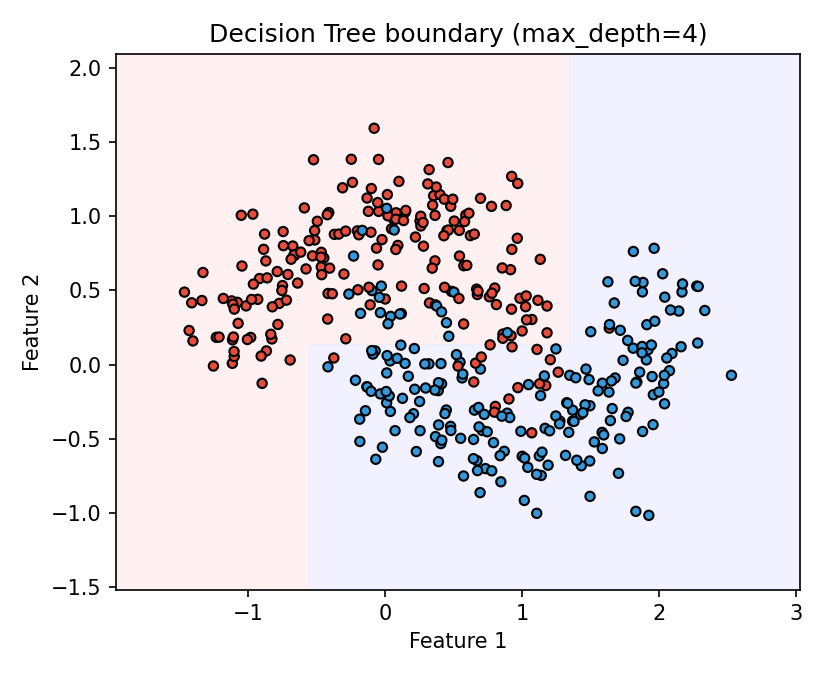
\includegraphics[width=0.9\linewidth]{dt_decision_boundary_2class.png}
  \caption{Decision tree decision boundary on a 2-class dataset.}
  \label{fig:dt2}
\end{figure}
\FloatBarrier

\begin{figure}[H]
  \centering
  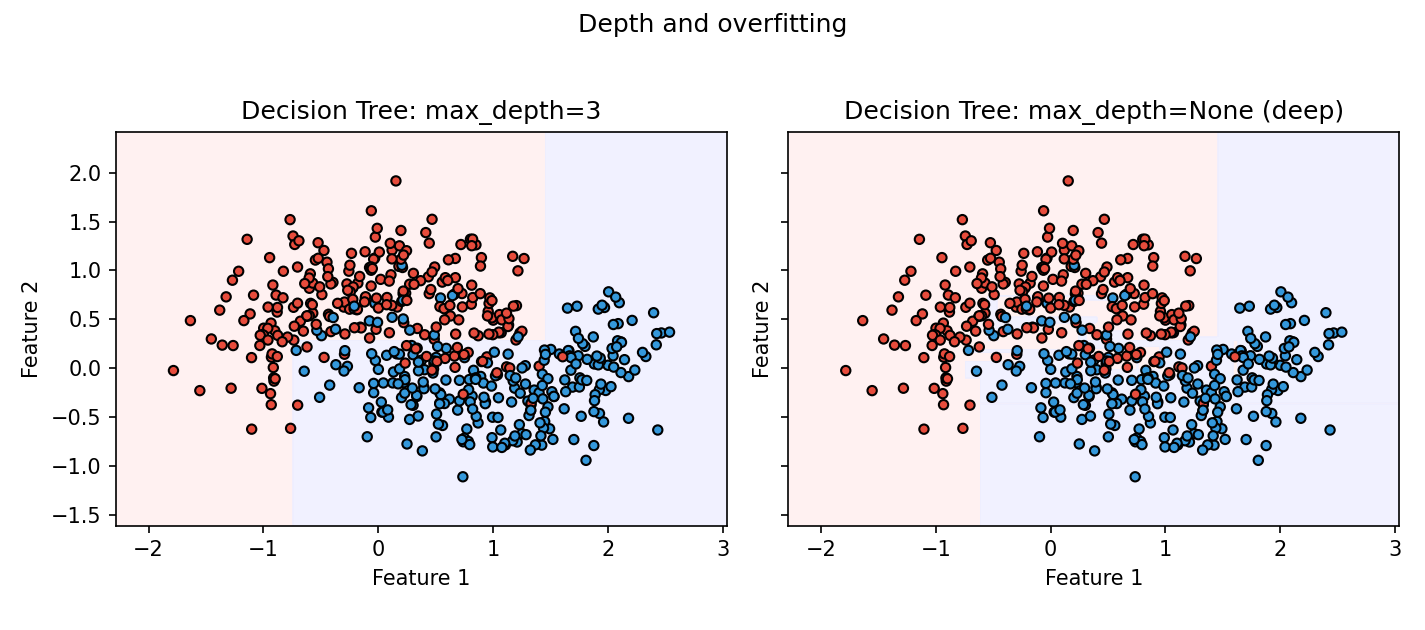
\includegraphics[width=0.95\linewidth]{dt_depth_compare.png}
  \caption{Effect of depth: shallow vs deep tree (overfitting).}
  \label{fig:depth}
\end{figure}
\FloatBarrier

\begin{figure}[H]
  \centering
  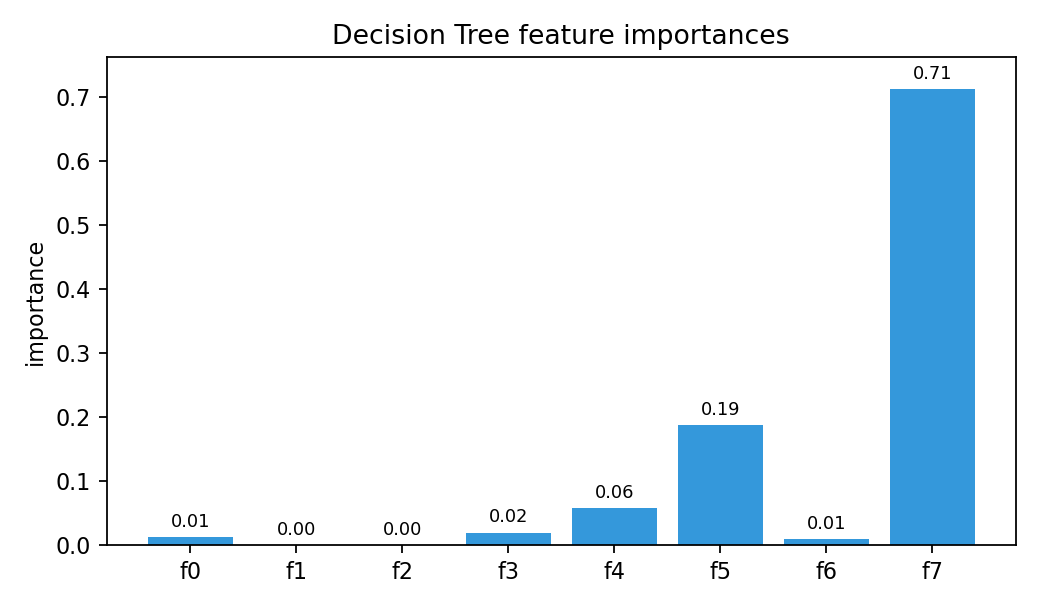
\includegraphics[width=0.85\linewidth]{dt_feature_importances.png}
  \caption{Feature importances from a decision tree.}
  \label{fig:fi}
\end{figure}
\FloatBarrier

\begin{figure}[H]
  \centering
  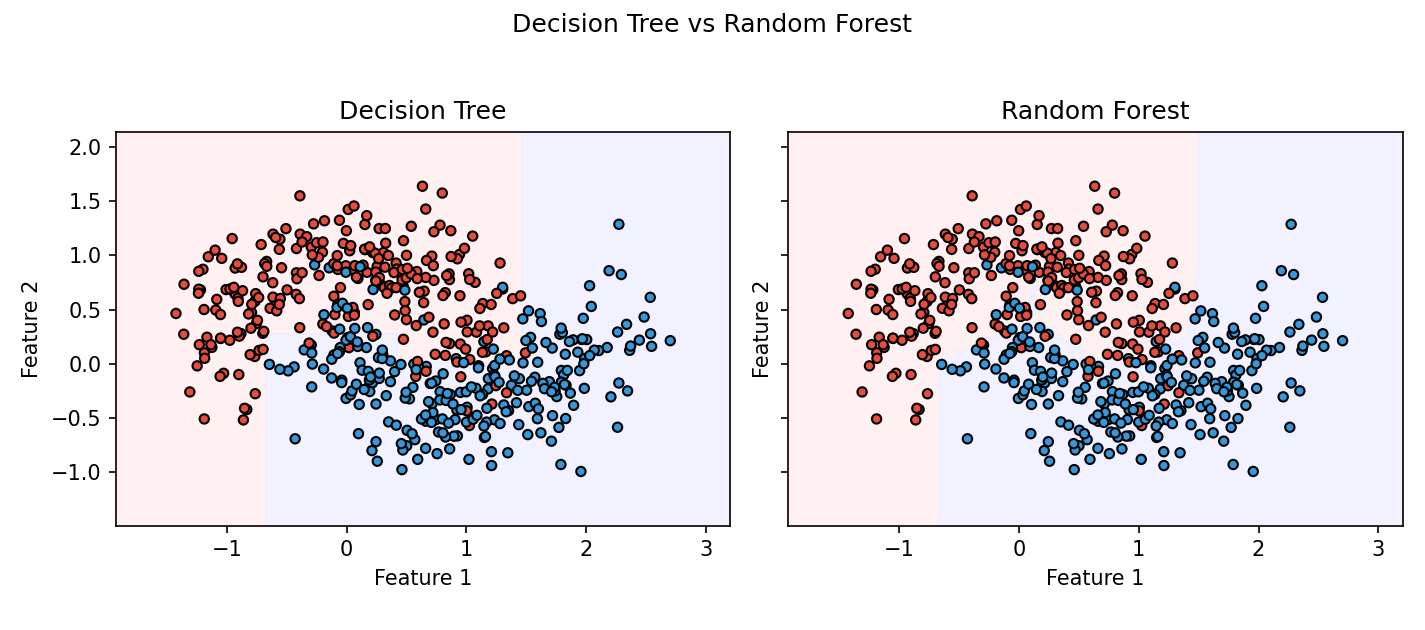
\includegraphics[width=0.95\linewidth]{dt_vs_rf_boundary.png}
  \caption{Decision boundary: single tree vs random forest.}
  \label{fig:dt_vs_rf}
\end{figure}
\FloatBarrier

\begin{figure}[H]
  \centering
  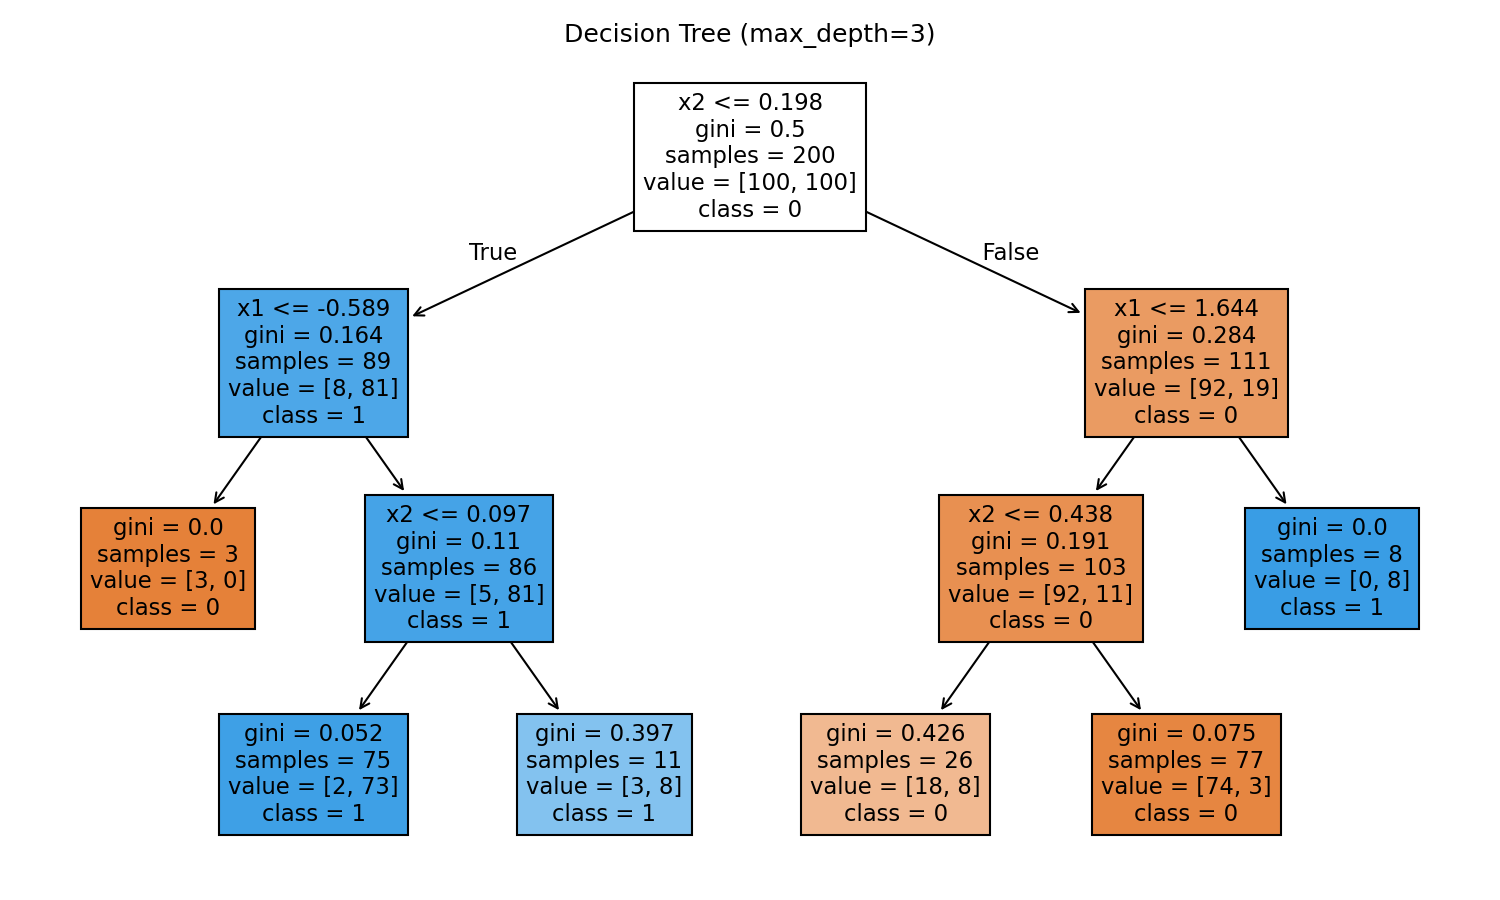
\includegraphics[width=0.95\linewidth]{dt_tree_plot.png}
  \caption{Tree structure visualization (max\_depth=3).}
  \label{fig:treeplot}
\end{figure}
\FloatBarrier

\section{Summary}
Decision trees provide interpretable, flexible baselines. With appropriate regularization or by using ensembles (random forests, gradient boosting), they become powerful general-purpose learners.

\end{document}
